\documentclass{article}
\usepackage[T1]{fontenc}
\usepackage{lmodern}
\usepackage[a4paper, landscape, margin=12mm]{geometry}
\usepackage{xcolor}
\usepackage{tikz}
\usepackage{array}
\usepackage{booktabs}

% One colour per course.
\definecolor{ttmath}{HTML}{4361EE}
\definecolor{ttphys}{HTML}{F72585}
\definecolor{ttchem}{HTML}{4CC9F0}
\definecolor{tthist}{HTML}{F8961E}
\definecolor{ttlang}{HTML}{43AA8B}
\definecolor{ttgrid}{HTML}{2B2D42}

% First and last hour shown in the grid (24 hour clock).
\newcommand{\firsthour}{8}
\newcommand{\lasthour}{17}

\renewcommand{\familydefault}{\sfdefault}
\pagestyle{empty}
\setlength{\parindent}{0pt}

% \lesson{day 1 to 5}{start}{end}{colour}{course}{room}. Use 9.5 for 9:30.
\newcommand{\lesson}[6]{%
  \pgfmathsetmacro{\lx}{(#1-1)*34+1}
  \pgfmathsetmacro{\ly}{(#2-\firsthour)*16+0.6}
  \pgfmathsetmacro{\lh}{(#3-#2)*16-1.2}
  \fill[#4!18, rounded corners=2pt] (\lx,\ly) rectangle ++(32,\lh);
  \fill[#4] (\lx,\ly) rectangle ++(1.4,\lh);
  \node[anchor=north west, text width=28mm, font=\scriptsize, inner sep=0pt, align=left]
    at (\lx+3,\ly+1.5) {\textbf{#5}\\#6};
}

\begin{document}

{\fontsize{26}{30}\selectfont\bfseries\color{ttgrid} Spring Term 2027\par}
\vspace{1mm}
{\large\color{ttgrid!60} Timetable for Amira Hassan, Year 12 \hfill Term dates: 11 January to 26 March\par}
\vspace{4mm}

\begin{minipage}[t]{0.7\textwidth}
  \vspace{0pt}
  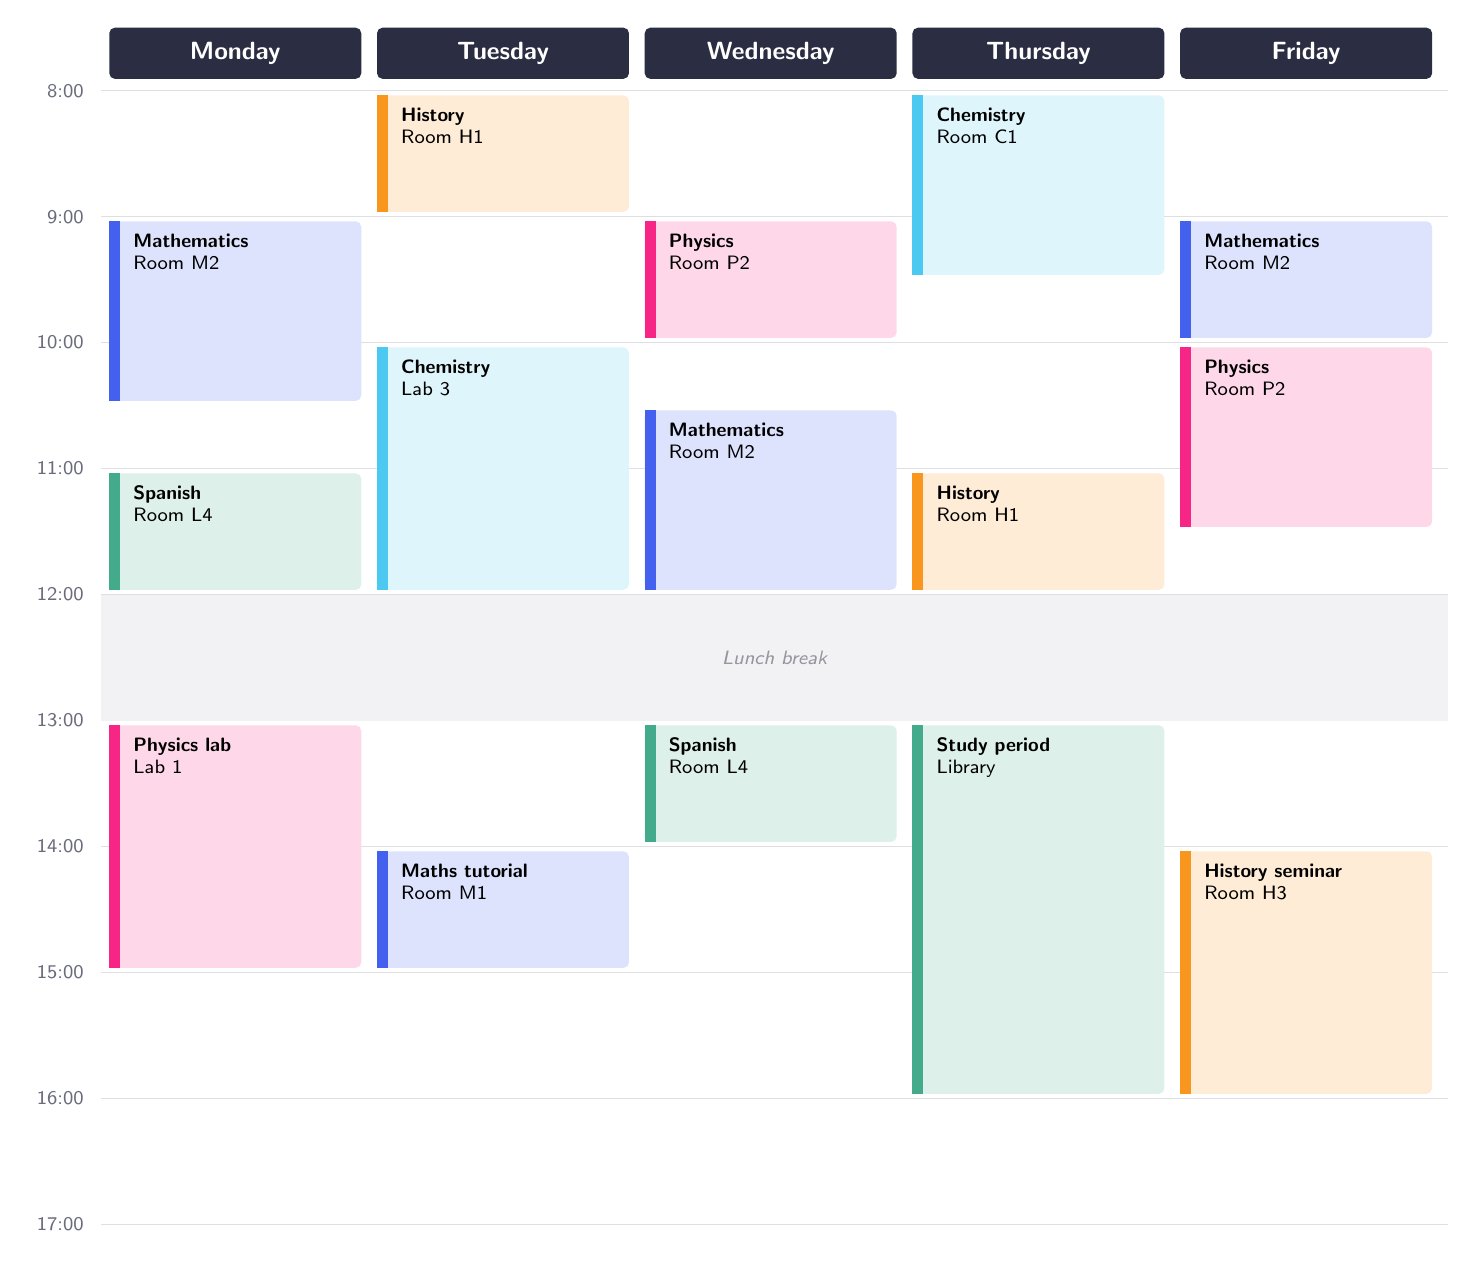
\begin{tikzpicture}[x=1mm, y=-1mm]
    % Day names across the top.
    \foreach \d [count=\i from 0] in {Monday,Tuesday,Wednesday,Thursday,Friday} {
      \fill[ttgrid, rounded corners=2pt] (\i*34+1,-8) rectangle ++(32,6.5);
      \node[text=white, font=\small\bfseries] at (\i*34+17,-4.75) {\d};
    }
    % Hour lines and labels.
    \pgfmathtruncatemacro{\nh}{\lasthour-\firsthour}
    \foreach \k in {0,...,\nh} {
      \pgfmathtruncatemacro{\hr}{\firsthour+\k}
      \draw[ttgrid!15] (0,\k*16) -- (171,\k*16);
      \node[anchor=east, font=\scriptsize, text=ttgrid!70] at (-1,\k*16) {\hr:00};
    }
    \fill[ttgrid!6] (0,4*16) rectangle (171,5*16);
    \node[font=\scriptsize\itshape, text=ttgrid!50] at (85.5,4.5*16) {Lunch break};

    % Lessons: edit, add or remove lines here.
    \lesson{1}{9}{10.5}{ttmath}{Mathematics}{Room M2}
    \lesson{1}{11}{12}{ttlang}{Spanish}{Room L4}
    \lesson{1}{13}{15}{ttphys}{Physics lab}{Lab 1}
    \lesson{2}{8}{9}{tthist}{History}{Room H1}
    \lesson{2}{10}{12}{ttchem}{Chemistry}{Lab 3}
    \lesson{2}{14}{15}{ttmath}{Maths tutorial}{Room M1}
    \lesson{3}{9}{10}{ttphys}{Physics}{Room P2}
    \lesson{3}{10.5}{12}{ttmath}{Mathematics}{Room M2}
    \lesson{3}{13}{14}{ttlang}{Spanish}{Room L4}
    \lesson{4}{8}{9.5}{ttchem}{Chemistry}{Room C1}
    \lesson{4}{11}{12}{tthist}{History}{Room H1}
    \lesson{4}{13}{16}{ttlang}{Study period}{Library}
    \lesson{5}{9}{10}{ttmath}{Mathematics}{Room M2}
    \lesson{5}{10}{11.5}{ttphys}{Physics}{Room P2}
    \lesson{5}{14}{16}{tthist}{History seminar}{Room H3}
  \end{tikzpicture}
\end{minipage}\hfill
\begin{minipage}[t]{0.26\textwidth}
  \vspace{0pt}
  {\bfseries\color{ttgrid} Key dates\par}
  \vspace{2mm}
  \small
  \renewcommand{\arraystretch}{1.35}
  \begin{tabular}{@{}>{\bfseries}l l@{}}
    \toprule
    11 Jan & First day of term \\
    25 Jan & Coursework 1 due \\
    15 Feb & Half term, one week \\
    1 Mar & Mock exams begin \\
    12 Mar & Parents' evening \\
    26 Mar & Last day of term \\
    \bottomrule
  \end{tabular}

  \vspace{6mm}
  {\normalsize\bfseries\color{ttgrid} Courses\par}
  \vspace{2mm}
  \newcommand{\swatch}[1]{\tikz\fill[#1, rounded corners=1pt] (0,0) rectangle (3mm,3mm);\ }
  \begin{tabular}{@{}l l@{}}
    \swatch{ttmath} Mathematics & Mr. Osei \\
    \swatch{ttphys} Physics & Dr. Lund \\
    \swatch{ttchem} Chemistry & Ms. Park \\
    \swatch{tthist} History & Mr. Byrne \\
    \swatch{ttlang} Spanish & Sra. Ruiz \\
  \end{tabular}

  \vspace{6mm}
  {\normalsize\bfseries\color{ttgrid} Notes\par}
  \vspace{2mm}
  \foreach \n in {1,...,5} {\rule{\linewidth}{0.3pt}\par\vspace{5mm}}
\end{minipage}

\end{document}
